\documentclass[10pt,fleqn]{article} % Default font size and left-justified equations
\usepackage[%
    pdftitle={Introduction à l'algorithmique et à la programmation},
    pdfauthor={Xavier Pessoles}]{hyperref}

\newcommand{\repRel}{../../../..}
\input{\repRel/Style/packages}
\input{\repRel/Style/new_style}
\input{\repRel/Style/macros_SII}
\input{\repRel/Style/environment}


\newcommand{\macrocomp}{macro_competences}
\newcommand{\comp}{competences}
\newcommand{\td}{fichier_td}
\newcommand{\repExo}{dossier}
\newcommand{\repStyle}{\repRel/Style}

\def\xxYCartouche{-2.25cm}
\def\xxYongletGarde{.5cm}
\def\xxYOnget{.9cm}

\begin{document}

\livrettrue
\graphicspath{{\repStyle/png/}}
\input{\repStyle/Info_01_Entete}
\graphicspath{{\repStyle/png/}{\repRel/Informatique/Semestre_01/01_Bases/Cours/images/}}
%\input{\repRel/Informatique/Semestre_01/01_Bases/Cours/01_Bases.tex}


\def\xxcompetences{}
\def\xxfigures{}
\def\xxchapitre{}
\def\xxtitreexo{Résolution d'équations différentielles -- Euler}
\def\xxsourceexo{}
\def\xxactivite{TP 11 -- BIS \ifprof  -- Corrigé \else \fi}
\input{\repRel/Style/pagegarde_TD}


\proffalse
\vspace{5cm}
\pagestyle{fancy}
\thispagestyle{plain}

\graphicspath{{\repStyle/png/}{\repRel/Informatique/Exercices/S1_07_Images/01_TraitementPGM/}}
%\input{\repRel/Informatique/Exercices/S1_07_Images/01_TraitementPGM.tex}


%
%\activite{Recherche d'un plus court chemin par un algorithme glouton}
%Commencez par télécharger la trame du fichier \texttt{.py} sur le site de la classe : 
%\url{https://mpsilamartin.github.io/info/TP/08_RechercheChemin.py}.


%\activite{Tracé de fonctions simples}

\graphicspath{{\repStyle/png/}{\repRel/Informatique/Exercices/S2_09_Dictionnaires/01_Snake_Ladders/}}
%\input{\repRel/Informatique/Exercices/S2_09_Dictionnaires/01_Snake_Ladders}


\section{Principe de la méthode de la méthode d'Euler}

Soit $y$ l'unique solution de
$$\begin{cases}
	y'(t)=F(t,y(t))\\y(t_0)=y_0
\end{cases} \quad \text{ avec $(t_0,y_0)$ fixé.}
$$


On souhaite obtenir une approximation de la fonction $y$ sur l'intervalle $[a,b]$.

Soit $n\in\N^*$. 

\begin{itemize}
\item  On découpe l'intervalle $[a,b]$ en $n$ sous-segments de même longueur $h= \dfrac{b-a}{n}$.
\item On pose : $ t_0=a \quad t_1= t_0+h \quad t_2= t_0+2h\quad \dots \quad t_k= t_0+kh \quad t_n= t_0+nh=b$.
%	\[t_0= a}\quad t_1= t_0+h}\quad t_2= t_0+2h}\quad \dots \quad t_k= t_0+kh}\quad t_n= t_0+nh=b}\]
	On part de $t_0$.
	\item On approche la portion de courbe entre $t_0$ et $t_1$ par la tangente à la courbe au point d'abscisse $t_0$.	
	\vskip1cm\begin{minipage}{0.5\linewidth}
		\begin{center}
			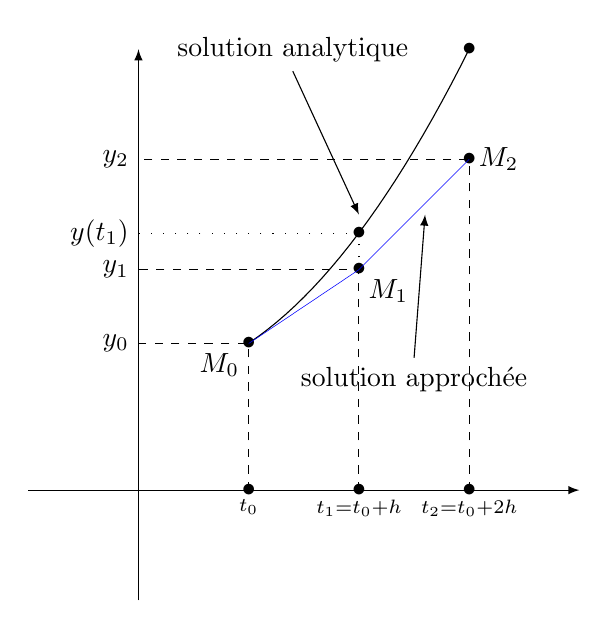
\begin{tikzpicture}[scale=1.4]
				\shorthandoff{:};
				\draw[->,>=latex] (-1,0)--(4,0);
				\draw[->,>=latex] (0,-1)--(0,4);
				\draw[domain=1:3] plot(\x,\x^2/3+1);
				\coordinate (A) at (1,1.33);
				\coordinate (B) at (2,2);
				\coordinate (C) at (3,3);
				\draw[dashed] (1,0)|-(0,1.33)node[left]{$y_0$};
				\draw (1,0) node{$\bullet$}node[below]{$\scriptstyle t_0$};
				\draw[dashed] (2,0)|-(0,2)node[left]{$y_1$};
				\draw (A) node{$\bullet$}node[below left]{$M_0$};
				\draw (B) node{$\bullet$}node[below right]{$M_1$};
				\coordinate (D) at(2,2.33);
				\draw(D)node{$\bullet$};
				\draw[loosely dotted](B)|-(0,2.33);
				\draw(0,2.33)node[left]{$y(t_1)$};
				\draw (C)node{$\bullet$}node[right]{$M_2$};
				\draw (3,4)node{$\bullet$};
				\draw (2,0) node{$\bullet$}node[below]{$\scriptstyle t_1=t_0+h$};
				\draw[dashed] (3,0)|-(0,3)node[left]{$y_2$};
				\draw (3,0) node{$\bullet$}node[below]{$\scriptstyle t_2=t_0+2h$};
				\draw[help lines,color=blue] (A)--(B)--(C);
				\node (solex) at (1.4,4){solution analytique};
				\node (solap) at (2.5,1){solution approchée};
				\draw[->,>=latex] (solex.south)--(2,2.5);
				\draw[->,>=latex] (solap.north)--(2.6,2.5);
			\end{tikzpicture}
		\end{center}
		\shorthandon{:}
	\end{minipage}\begin{minipage}{0.5\linewidth}
		
		Le point $M_1(t_1,y_1)$ appartient à la tangente à la courbe au point $M_0(t_0,y_0)$.\\
		Alors,   {$y'(t_0) \approx \displaystyle\frac{y_1-y_0}{h}$}
		D'où, $y_1=y_0+hy'(t_0)$.\\
		Soit encore,   {$y_1=y_0+hF(t_0,y_0)$.}\\
		$y_1$ est une valeur approchée de la valeur exacte $y(t_1)$.
		
	\end{minipage}
	
	
	%On recommence le procédé à partir du point $M_1(t_1,y_1)$.
	
	\item De manière générale, on pose:
%	\begin{framed}
$\forall k\in\{0,\dots,n-1\},\quad  y_{k+1}=y_k+hF(t_k,y_k)$
. %\] %\end{framed}	
	Ce qui amène à construire successivement les points $M_k$ de coordonnées $(t_k,y_k)$. La ligne polygonale reliant ces points est alors une approximation de la courbe représentative de la solution.
\end{itemize}

\subsection{Programmation de la méthode }

\question{Considérant l'équation différentielle d'ordre 1 $y'(t)=F(t,y(t))$, écrire en python une fonction \texttt{Euler(F, a, b, n)} d'arguments la fonction $F$, les bornes $a$ et $b$ de l'intervalle d'étude, la condition initiale $y0$ et le nombre d'étapes $n$. Cette fonction renverra une liste de temps et une liste de valeurs approchées par la méthode d'Euler.}
	
\question{Tracer la solution analytique et la solution approchée donnée par la méthode d'Euler pour l'équation différentielle:$$y'(t)+ty(t)=0$$ avec $y(0)=1$. On prendra $a=0$, $b=1$, $n=100$.}

\subsection{Application}

Dans cet exercice, on souhaite étudier une fonction $t\mapsto y(t)$ sur un intervalle $[a,b]$. La fonction $y$ est solution de l'équation différentielle $y''=-\displaystyle\frac 1{y^2}$ avec les conditions initiales $y(a)=y0 \textrm{ et } y'(a)=yp0.$

\question{Mettre l'équation différentielle considérée sous forme d'un système de deux équations différentielles du premier ordre en introduisant une fonction auxilliaire $z(t)=y'(t)$.}
	
\question{Compte tenu du système d'équations différentielles, comment exprimer $z(t+h)$ et $y(t+h)$ en fonction de $h$, $y(t)$ et $z(t)$ (ou $h$ est la pas de la subdivision) ?}
	
%\bigskip
 On souhaite résoudre l'équation différentielle  sur l'intervalle $[a,b]$ en utilisant $N$ intervalles, soit $N+1$ points du segment $[a,b]$ (le premier vaut $a$, le dernier vaut $b$).

\question{En supposant $N$, $a$ et $b$ préalablement définis dans le programme, écrire des lignes de code pour calculer le pas \texttt{h} ainsi que la liste \texttt{les\_t} des $N+1$ instants équirépartis entre $a$ et $b$.}
	
\question{\'Ecrire une fonction \texttt{euler2(a,b,N,y0,yp0)} qui calcule et renvoie les listes \texttt{les\_t}, \texttt{les\_y} et \texttt{les\_z} correspondant aux différents instants et aux valeurs approximées par la \textbf{méthode d'Euler} des fonctions $y$ et $z$ à ces différents instants.}
	

On peut montrer (la justification n'est pas demandée ici) à l'aide de développements limités à l'ordre 2 que $$y(t+h)-2y(t)+y(t-h)=y''(t).h^2+O(h^3).$$
Une méthode appelée \textbf{méthode de Verlet} consiste à négliger le terme en $O(h^3)$ et à écrire:
$$y(t+h)-2y(t)+y(t-h)=y''(t).h^2.$$

\question{Compte tenu de l'approximation de la méthode de Verlet et de l'équation différentielle, exprimer $y(t+h)$ en fonction de $y(t)$, $y(t-h)$ et $h$ uniquement.}
	
\question{Pourquoi ne peut-on pas utiliser cette expression pour le calcul du premier point (c'est-à-dire pour le calcul de $y$ en $t_1=a+h$) ?}
	
\question{A l'aide d'un développement limité à l'ordre 2 et en négligeant le terme en $O(h^3)$, exprimer $y(a+h)$ en fonction de $h, y0, yp0$ et $y''(a)$.}
	
\question{En tenant compte de l'équation différentielle, modifier l'expression précédente pour exprimer $y(a+h)$ en fonction de $h, y0, yp0$ uniquement.}
	
\question{Ecrire une fonction \texttt{verlet(a,b,N,y0,yp0)} qui calcule et renvoie les listes \texttt{les\_t}, \texttt{les\_y}, \texttt{les\_z} par la méthode de Verlet.}
	

 Pour comparer les méthodes, on se propose de trouver une intégrale première du mouvement. Pour cela, on multiplie l'équation différentielle par $y'$ et on prend une primitive.

\question{Montrer que $E(t)=\displaystyle\frac 12 y'(t)^2-\displaystyle\frac 1{y(t)}$ est une constante (indépendante de $t$).}
	
\question{Ecrire les lignes de code permettant de tracer la courbe $E(t)$ obtenue avec la méthode d'Euler et celle obtenue avec la méthode de Verlet sur le même graphique ($a=0, b=20, y0=10, yp0=0.03$ et on se limitera à une graduation des ordonnées comprise entre -0.1 et -0.0975)} 
	





\end{document}



